In our formal analysis, we deliberately focused on highlighting various snapshots that capture the intricate representation of the system, opting against the utilization of Alloy 6's time features. This strategic decision stems from our dedication to modeling the inherent complexity of the problem in a more comprehensive manner. The incorporation of Alloy 6 features would have presented substantial challenges, given the heightened complexity they introduce. Moreover, it would have necessitated a compromise in the completeness of our representation, as it would require reducing the intricacy to accommodate the depiction of time evolution.

\section{Alloy Code}
\lstinputlisting[language=alloy]{alloy/CKB_alloy.als}

\section{Assertion Results}

\begin{figure}[H]
    \centering
    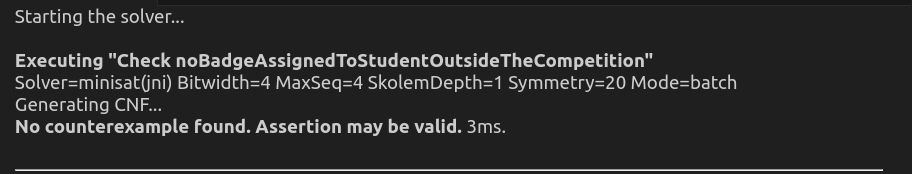
\includegraphics[width=200px]{Images/alloy/assert_1.png}
    \caption{assert there is no student part of a battle for a competition it did not join}
\end{figure}

\begin{figure}[H]
    \centering
    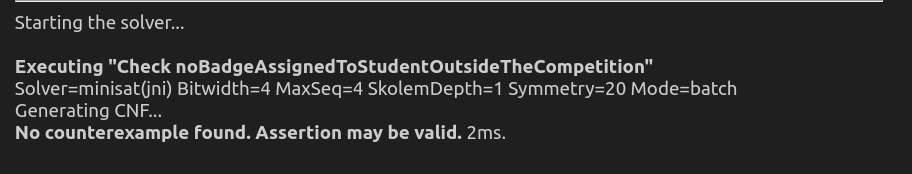
\includegraphics[width=200px]{Images/alloy/assert_2.png}
    \caption{assert there is no started battle with waiting teams inside}
\end{figure}

\begin{figure}[H]
    \centering
    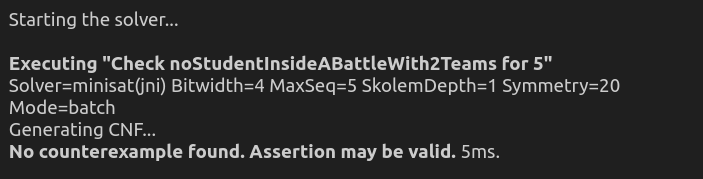
\includegraphics[width=200px]{Images/alloy/assert_3.png}
    \caption{assert there is no student isnide a battle with 2 teams}
\end{figure}


\begin{figure}[H]
    \centering
    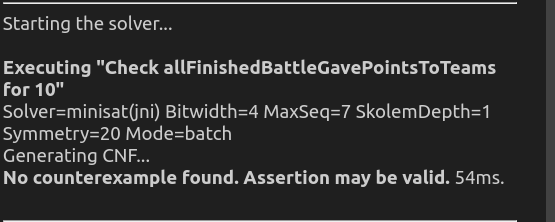
\includegraphics[width=200px]{Images/alloy/assert_4.png}
    \caption{assert all finish battle gave points to the teams}
\end{figure}

\section{World Generated}
